% !TEX root = ../msimplicial.tex

\section{Multisimplicial algebraic topology}

\subsection{Multisimplicial sets}

Let us consider an arbitrary non-negative integer~$k$.
The \textit{$k$-fold multisimplex category} $\simplex^{\times k}$ is the $k$-fold Cartesian product of the simplex category $\simplex$, with the convention that for $k = 0$ this is the trivial category.
The category of \textit{multisimplicial sets} is the coproduct
\[
\mSet = \coprod_{k \in \N} \mSet^{(k)}
\]
where $\mSet^{(k)}$ denotes the category of presheaves $\Fun \big( (\simplex^{\times k})^\op, \Set \big)$, whose objects are referred to as \textit{$k$-fold multisimplicial sets}.
The categories $\mSet^{(0)}$ and $\mSet^{(1)}$ are naturally equivalent to $\Set$ and $\sSet$ respectively.
The representable $k$-fold multisimplicial sets are denoted by
\[
\simplex^{n_1,\dots,n_k} =
\yoneda \big([n_1]\times\dots\times[n_k]\big)
\]
and we have
\[
\simplex^{n_1,\dots,n_k} \big([m_1]\times\dots\times[m_k]\big) \cong
\simplex^{n_1}_{m_1}\times\dots\times\simplex^{n_k}_{m_k}.
\]
Explicitly, a $k$-fold multisimplicial set $X$ consists of a collection of sets
\[
X_{m_1,\dots,m_k} =
X \big( [m_1] \times\dots\times [m_k] \big)
\]
indexed by tuples of non-negative integers $(m_1,\dots,m_k)$ together with \textit{face maps}
\[
\face_i^j \colon
X_{m_1, \dots, m_j,\dots,m_k} \to
X_{m_1, \dots, m_j-1, \dots, m_k}
\]
and \textit{degeneracy map}
\[
\dege^j_i \colon X_{m_1, \dots, m_j,\dots,m_k} \to X_{m_1, \dots, m_j+1, \dots, m_k}
\]
for $1 \leq j \leq k$ and $0 \leq i \leq m_j$ such that, referring to $j$ as the \textit{direction} of these maps, two of them satisfy the simplicial identities when they have the same direction and commute when they do not.
An element of $X_{m_1,\dots,m_k}$ is called
$(m_1,\dots,m_k)$-\textit{multisimplex}.
A multisimplex is \textit{degenerate} if it is in the image of a degeneracy map.

\subsection{Geometric realization}

We will use the following model of the topological simplex:
\[
\gsimplex^n = \big\{
(t_1, \dots, t_n) \in [0,1]^n \mid t_1 \geq \dots \geq t_n
\big\}
\]
with
\[
\delta_i(t_1, \dots, t_n) =
\begin{cases}
	(1, t_1, \dots, t_n) & i = 0, \\
	(t_1, \dots, t_i, t_i, \dots, t_n) & 0 < i < n, \\
	(t_1, \dots, t_n, 0) & i = n,
\end{cases}
\]
and
\[
\sigma_i(t_1, \dots, t_n) = (t_1, \dots, \widehat t_i, \dots, t_n).
\]
The \textit{geometric realization} functor
\[
\bars{-} \colon \mSet \to \Top
\]
is defined as the Yoneda extension of the functor defined on representable objects by
\[
\bars{\simplex^{n_1,\dots,n_k}} =
\gmsimplex{n_1}{n_k}
\]
Explicitly, for a $k$-fold multisimplicial set $X$ we have
\begin{align*}
	\bars{X} &\cong
%	\colim_{\cramped{(\simplex^{n_1,\dots,n_k} \downarrow X})} \, \bars{\simplex^{n_1,\dots,n_k}} \\ &=
	\coprod \gmsimplex{n_1}{n_k} \times X_{n_1,\dots,n_k} /_\sim
\end{align*}
where
\[
\begin{split}
	(t_1, \dots, t_j, \dots, t_k, \face^j_i(x)) &\sim (t_1, \dots, \delta_i(t_j), \dots, t_k, x), \\
	(t_1, \dots, t_j, \dots, t_k, \dege^j_i(x)) &\sim (t_1, \dots, \sigma_i(t_j), \dots, t_k, x), \todo{@paolo: I don't think this is right. Is $t_i$ a real number? It seems its a vector.}
\end{split}
\]
which equips $\bars{X}$ with a canonical cellular structure.

As expected, the restriction of the geometric realization functor to the subcategory of $1$-fold multisimplicial sets recovers the usual geometric realization of simplicial sets up to natural equivalence.

The restriction of the geometric realization functor to $k$-fold multisimplicial sets has a right adjoint
\[
\Sing^{(k)} \colon \Top \to \mSet^{(k)}
\]
defined on a topological space $\fZ$, as usual, by the expression
\[
\Sing^{(k)}(\fZ)_{n_1,\dots,n_k} = \Top(\gmsimplex{n_1}{n_k},\fZ).
\]

\todo{@everyone: Quillen equivalence}

\subsection{Algebraic realization}

The functor of \textit{chains}
\[
\chains \colon \mSet \to \Ch,
\]
is the Yoneda extension of the functor defined on representable objects by
\[
\chains \big( \simplex^{n_1, \dots, n_k} \big) =
\chains(\simplex^{n_1}) \ot \dotsb \ot \chains(\simplex^{n_k}).
\]
It is naturally isomorphic to the composition of the geometric realization functor and the functor of cellular chains with respect to the canonical cellular structure.

Explicitly, for a $k$-fold multisimplicial set $X$ the $\k$-module $\chains(X)_n$ is freely generated by the non-degenerate $(n_1, \dots, n_k)$-multisimplices $x$ with $n_1+\dots+n_k = n$ and differential given by
\[
d(x) = \sum_{j=1}^k \sum_{\ell_j=1}^{n_j}
(-1)^{n_{1}+\dots+n_{j-1}+\ell_j} \, d^j_{\ell_j}(x).
\]

\begin{remark*}
	If we do not mod out by degenerate multisimplices the same formula defines the functor of \textit{non-normalized chains}.
	A slight generalization of the classical normalization theorem by MacLane \cite{MacLane} shows that the natural projection between these is a natural chain homotopy equivalence. \todo{@andrea: please get the missing reference.}
\end{remark*}

For any topological space $\fZ$ the complex of chains of $\Sing^{(k)}(\fZ)$ is denoted $\rS^{(k)}(\fZ)$ and referred to as the $k$-\textit{fold singular chains} of $\fZ$.

\subsection{Alexander--Whitney structure}

Recall that a \textit{counital coalgebra} consists of a chain complex $C$ and chain maps $\copr \colon C \to C \ot C$ and $\aug \colon C \to \k$ satisfying
\[
(\id \ot \aug) \circ \copr =
\id =
(\aug \ot\, \id) \circ \copr.
\]
For each integer $n$ the chain complex $\chains(\simplex^n)$ is naturally a counital coalgebra with structure maps defined by:
\[
\begin{split}
	\copr \big( [v_0, \dots, v_m] \big) &=
	\sum_{i=0}^m \, [v_0, \dots, v_i] \ot [v_i, \dots, v_m], \\
	\aug \big( [v_0, \dots, v_q] \big) &=
	\begin{cases} 1 & \text{ if } q = 0, \\ 0 & \text{ if } q>0. \end{cases}
\end{split}
\]
The tensor product of two coalgebras $C$ and $C'$ is a coalgebra with structure maps given by the compositions:
\begin{gather*}
	C \ot C^\prime \xra{\copr \ot \copr^\prime}
	(C \ot C) \ot (C^\prime \ot C^\prime) \xra{(23)}
	(C \ot C^\prime) \ot (C \ot C^\prime), \\
	C \ot C^\prime \xra{\aug \ot \aug^\prime}
	\k \ot \k \xra{\cong} \k.
\end{gather*}
From these constructions one deduces a natural counital coalgebra structures on the chains of representable multisimplicial sets $\chains \big( \simplex^{n_1, \dots, n_k} \big) = \chains(\simplex^{n_1}) \ot \dotsb \ot \chains(\simplex^{n_k})$, and, via a Yoneda extension, one on the chains of general multisimplicial sets.
Explicitly, for a $k$-fold multisimplicial set $X$ and $(m_1,\dots,m_k)$-multisimplex $x$ let
\[
\fI_{m_1,\dots,m_k} = \set[\big]{(i_{1},\dots,i_{k}) \mid 0 \le i_j \le m_j,\ \forall j = 1,\dots,k},
\]
then
\[
\copr(x) =
\sum_{I\in \mathfrak{I}_{k,x}} \;
(-1)^{\sum_{1 \leq l<h \leq k} i_h (m_l-i_l) } \
x \rfloor_{(i_{1},\dots,i_{k})} \ot
\!\,_{(m_{1}-i_{1}, \dots, m_{k}-i_{k})} \lfloor x
\]
where the \textit{front $(i_1,\dots,i_k)$-face} of $x$ is the multisimplex
\[
x \rfloor_{(i_{1}, \dots, i_{k})} =
X(F_{i_1}, \dots, F_{i_k})(x) \in X_{i_1,\dots,i_k}
\]
with
$F_{i_j} \colon [i_j] \to [n_j]$ defined by $F_{i_j}(h)=h$, and the \textit{back $(i_1,\dots,i_k)$-face} of $x$ is the multisimplex
\[
\,_{(i_{1}, \dots, i_{k})} \lfloor x =
X(B_{i_1}, \dots, B_{i_k})(x) \in X_{i_1,\dots,i_k}
\]
with $B_{i_j} \colon [i_j] \to [n_j]$ defined by $B_j(h) = h+m_j-i_j$.

\subsection{\pdfEinfty-extension}

An \textit{$\cM$-bialgebra} is a counital coalgebra $(C, \copr, \aug)$ together with a degree $1$ linear map $\pr \colon C \ot C \to C$ whose boundary is $(\aug \ot \id) - (\id \ot \aug)$ and such that $\aug \circ \pr = 0$.
As proven in \cite{medina2020prop1}, the collection of all maps $\set{C \to C^{\ot r}}_{r \in \N}$ generated by $\copr$, $\aug$ and $\pr$ make $C$ into an $E_\infty$-coalgebra, that is to say, a coalgebra over an $\sym$-free resolution of the terminal operad.

For any integer $n$, the \textit{join product} $\ast \colon \chains(\simplex^n)^{\ot 2} \to \chains(\simplex^n)$ is the natural degree~$1$ linear map defined by
\begin{equation*}
	\left[v_0, \dots, v_p \right] \pr \left[v_{p+1}, \dots, v_q\right] =
	\begin{cases} (-1)^{p} \sign(\pi) \left[v_{\pi(0)}, \dots, v_{\pi(q)}\right] & \text{ if } v_i \neq v_j \text{ for } i \neq j, \\
		\hfil 0 & \text{ if not}, \end{cases}
\end{equation*}
where $\pi$ is the permutation that orders the vertices.
It is an algebraic version of the usual join of faces in a simplex, as illustrated in \cref{f:join of faces}.
It is proven in \cite{medina2020prop1} that for any integer $n$ the counital coalgebra $\chains(\simplex^n)$ forms with the join product a natural $\cM$-bialgebra and, consequently, a natural $E_\infty$-coalgebra.

\begin{figure}
	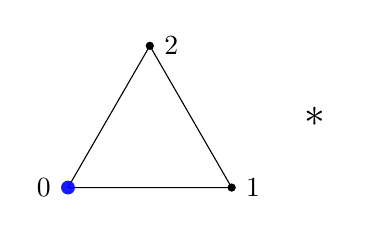
\begin{tikzpicture}[scale=.6]
\coordinate (A) at (210:2);
\coordinate (B) at (-30:2);
\coordinate (C) at (90:2);

\draw[draw=black] (A) -- (B) -- (C) -- (A);

\node[circle,fill=blue, opacity=.9, inner sep=0pt,minimum size=5pt, label=left:{0}] (a) at (A) {};
\node[circle,fill=black,inner sep=0pt,minimum size=3pt, label=right:{$1$}] (a) at (B) {};
\node[circle,fill=black,inner sep=0pt,minimum size=3pt, label=right:{$2$}] (a) at (C) {};

\node[scale=1.5] at (3.5,0.5) {$\ast$};
\end{tikzpicture}
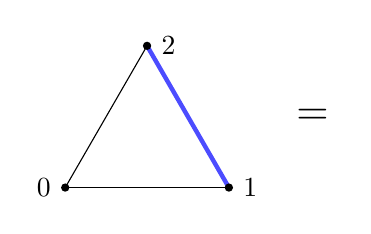
\begin{tikzpicture}[scale=.6]
\coordinate (A) at (210:2);
\coordinate (B) at (-30:2);
\coordinate (C) at (90:2);

\draw[draw=blue, ultra thick, draw opacity=.7] (B) -- (C);
\draw[draw=black] (C) -- (A);
\draw[draw=black] (A) -- (B);

\node[circle,fill=black,inner sep=0pt,minimum size=3pt, label=left:{$0$}] (a) at (A) {};
\node[circle,fill=black,inner sep=0pt,minimum size=3pt, label=right:{$1$}] (a) at (B) {};
\node[circle,fill=black,inner sep=0pt,minimum size=3pt, label=right:{$2$}] (a) at (C) {};

\node[scale=1.5] at (3.5,.5) {=};
\end{tikzpicture}
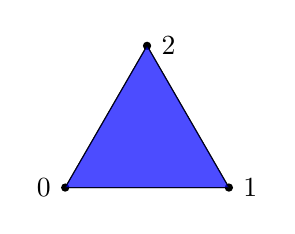
\begin{tikzpicture}[scale=.6]
\coordinate (A) at (210:2);
\coordinate (B) at (-30:2);
\coordinate (C) at (90:2);

\draw[draw=black] (A) -- (B) -- (C) -- (A);

\node[circle,fill=black,inner sep=0pt,minimum size=3pt, label=left:{$0$}] (a) at (A) {};
\node[circle,fill=black,inner sep=0pt,minimum size=3pt, label=right:{$1$}] (a) at (B) {};
\node[circle,fill=black,inner sep=0pt,minimum size=3pt, label=right:{$2$}] (a) at (C) {};

\draw[draw, fill=blue, opacity=.7] (A) -- (B) -- (C) -- (A);
\end{tikzpicture}
	\caption{Geometric representation of the join product of two basis elements. It depicts the identity $\big([0] \pr [1,2]\big) = [0,1,2]$.}
	\label{f:join of faces}
\end{figure}

Given two $\cM$-bialgebras, their tensor product $C \ot C^\prime$ is an $\cM$-bialgebra with structure map given by
\[
(C \ot C^\prime) \ot (C \ot C^\prime) \xra{(23)}
C \ot C \ot C^\prime \ot C^\prime
\xra{\aug \ot \id \ot \pr + \pr \ot \id \ot \aug}
C \ot C^\prime.
\]
Therefore, we obtain a natural $\cM$-bialgebra structure, and, consequently a natural $E_\infty$-coalgebra structure, on each $\chains \big( \simplex^{n_1, \dots, n_k} \big) = \chains(\simplex^{n_1}) \ot \dotsb \ot \chains(\simplex^{n_k})$.
We can extend this natural $E_\infty$-coalgebra structure to the chains on any multisimplicial set $X$.
Explicitly, \todo{@anibal: finish this}

We remark that, since the category of $\cM$-bialgebras is not cocomplete, we do not necessarily have an $\cM$-bialgebra structure on $\chains(X)$ for a general multisimplicial set $X$.
An example for which such structure does not exist is given one such $X$ whose geometric realization is isomorphic to two points.

\subsection{Steenrod cup-$(p,i)$ coproducts}

TBW\todo{@anibal: write this}

\subsection{Diagonal simplicial set} \label{ss:diagonal simplicial set}

The composition with the diagonal functor
\[
\simplex^\op \xra{\diag}
(\simplex^\op)^{\times k} \xra{\cong}
(\simplex^{\times k})^{\op}
\]
defines a functor
\[
(-)^{\diag} \colon \mSet \to \sSet
\]
explicitly defined on a $k$-fold multisimplicial set $X$ by
\begin{gather*}
	X^{\diag}_m = X_{m, \dots, m},
	\qquad
	\face_i = \face_i^1 \circ \dots \circ \face_i^k,
	\qquad
	\dege_i = \dege_i^1 \circ \dots \circ \dege_i^k.
\end{gather*}
It is straightforward to verify that
\[
\big(\simplex^{n_1,\dots,n_k}\big)^\diag \cong
\msimplex{n_1}{n_k}
\]
as simplicial sets.

The functor $(-)^\diag \colon \mSet \to \sSet$ admits a right adjoint $\radj \colon \sSet \to \mSet$, defined, as usual, by the expression
\[
\radj(Y)_{m_1,\dots,m_k} =
\sSet\big( \simplex^{m_1} \times \dots \times \simplex^{m_k}, \, Y \big).
\]
\todo{@everyone: we need a reference or a proof that they form a Quillen equivalence. This result is used for the zig-zag of $E_\infty$-q-iso. I would simply put a reference to the bisimplicial case in a remark like the one in the previous subsection, saying something similar.}

\subsection{Eilenberg--Zilber map}

Recall that an \textit{$(n_1,\dots,n_k)$-shuffle} $\sigma$ is a permutation in $\sym_n$ satisfying
\begin{gather*}
	\sigma(1) < \dots < \sigma(n_1), \\
	\sigma(n_1+1) < \dots < \sigma(n_1+n_2), \\
	\vdots \\
	\sigma(n-n_k-1) < \dots < \sigma(n),
\end{gather*}
where $n = n_1+\dots+n_k$.
We denote the set of such permutations by $\sh_{n_1,\dots,n_k}$.
For any $\sigma \in \sh_{n_1,\dots,n_k}$ the inclusion
\[
\gi_\sigma \colon \gsimplex^n \to \gmsimplex{n_1}{n_k}
\]
is defined by the assignment
\[
(x_1,\dots,x_n) \mapsto (x_{\sigma^{-1}(1)}, \dots, x_{\sigma^{-1}(n)}).
\]
If $e$ is the identity permutation, we denote $\gi_{e}$ simply as $\mathfrak{i}$.
The set $\set{\gi_\sigma \mid \sigma \in \sh_{n_1,\dots,n_k}}$ defines a triangulation of $\gmsimplex{n_1}{n_k}$ making it isomorphic, in the category cellular spaces, to the geometric realization of the simplicial set $\msimplex{n_1}{n_k}$.
Using this identification, the identity map induces a cellular map
\[
\ez \colon \gmsimplex{n_1}{n_k} \to \bars[\big]{\msimplex{n_1}{n_k}},
\]
whose induced chain map
\[
\EZ \colon \chains(\simplex^{n_1,\dots,n_k}) \to \chains\big(\msimplex{n_1}{n_k}\big),
\]
agrees, under the natural identifications, with the traditional Eilenberg--Zilber map.
For a multisimplicial set $X$, the induced chain map $\EZ \colon \chains(X) \to \chains(X^\diag)$ is defined on an $(n_1,\dots,n_k)$-multisimplex $x$ by
\[
\EZ(x) = \sum_{\sigma \in \sh_{n_1,\dots,n_k}} \sign(\sigma) \, X(\sigma_1 ,\dots, \sigma_k)(x) \todo{@anibal: use mathtools to fix display}
\]
%\[
%\EZ \big( [n_1] \times\dots\times [n_k] \big) =
%\sum_{\sigma \in \sh_{n_1,\dots,n_k}} \sign(\sigma) \, \sigma_1 \times\dots\times \sigma_k
%\]
where, for $\ell \in \set{1,\dots,k}$, the morphisms $\sigma_\ell \colon [n] \to [n_\ell]$ are defined by the following property: For
each $j \in \set{1,\dots,n}$ there is exactly one $\ell \in \set{1,\dots,k}$ such that $\sigma_\ell(j+1) = \sigma_\ell(j)+1$ and $\sigma_i(j+1) = \sigma_i(j)$ for all $i \neq \ell$.
\todo{@andrea: this is off, unfortunately. Could you please fix it?}

\begin{lemma}
	The map $\EZ$ is a coalgebra quasi-isomorphism. \todo{@anibal: finish this}
\end{lemma}

\begin{remark}
	But not a morphisms of $E_\infty$-coalgebras. \todo{@anibal: finish this}
\end{remark}

\subsection{Canonical inclusion}

Let $Y$ be a simplicial set and $n$ an integer.
Consider the function $Y_n \to \cU Y_{n,0,\dots,0}$ sending a simplex with characteristic map $\zeta \colon \simplex^n \to Y$ to the composition
\[
\simplex^n \times \msimplex{0}{0} \xra{\pi_1} \simplex^n \xra{\zeta_y} Y.
\]
These functions induce a chain map
\[
\In \colon \chains(Y) \to \chains(\cU Y)
\]
and we have the following.

\begin{lemma*}
	The canonical inclusion $\In \colon \chains(Y) \to \chains(\cU Y)$ is a quasi-isomorphism of $E_\infty$-coalgebras for any simplicial set $Y$.
\end{lemma*}

\begin{proof}
	The structure preserving properties of this map are immediate.
	It remains to be shown that it induces a homology isomorphism.
	Consider the composition
	\[
	\chains(\cU Y) \xra{\EZ}
	\chains\big((\cU Y)^\diag\big) \to
	\chains(Y)
	\]
	where the second map is induced by the counit of the adjunction.
	This composition is a quasi-isomorphism by ?? and ??.
	We will now verify that it is left inverse to $\In$.
	Consider a simplex $y$ with characteristic map $\zeta \colon \simplex^n \to Y$.
	The multisimplex $\In(y)$ is given by the simplicial map $\simplex^n \times \msimplex{0}{0} \xra{\pi_1} \simplex^n \xra{\zeta} Y$.
	Since the only $(n,0,\dots,0)$-shuffle is the identity, the simplex $\EZ \circ \In (y)$ is the simplicial map
	\[
	\zeta \circ \pi_1 \colon \simplex^n \times \msimplex{n}{n} \to Y.
	\]
	Finally, the image of this simplex under the counit is the evaluation of $[n] \times\dots\times [n]$ on $\zeta \circ \pi_1$ which gives $\zeta[n] = y$ as claimed.\todo{@anibal: add missing references.}
\end{proof}

\begin{corollary*}
	Let $\fZ$ be a topological space.
	The chain map
	\[
	\rS^{(1)}(\fZ) \to \rS^{(k)}(\fZ)
	\]
	defined by precomposing a continuous map $(\gsimplex^n \to \fZ)$ by the projection
	\[
	\gsimplex^n \times \gmsimplex{0}{0} \xra{\pi_1} \gsimplex^n
	\]
	is a quasi-isomorphism of $E_\infty$-coalgebras.
\end{corollary*}

\begin{proof}
	This map factors as the composition of two quasi-isomorphism of $E_\infty$-coalgebras.
	The first is $\In \colon \rS^{(1)}(\fZ) \to \chains(\cU^{(k)} \Sing^{(1)}(\fZ))$, which was studied in the previous lemma.
	The second is induced from a multisimplicial isomorphism
	\[
	\cU^{(k)} \Sing^{(1)}(\fZ) \to \Sing^{(k)}(\fZ)
	\]
	defined as follows.
	Using the adjunction of \cref{ss:geometric realization}, any simplicial map $\msimplex{n_1}{n_k} \to \Sing^{(1)}(\fZ)$ corresponds canonically to a continuous map $\bars{\msimplex{n_1}{n_k}} \to \fZ$, which precomposing with $\ez$ gives a continuous map $\gmsimplex{n_1}{n_k} \to \fZ$.
	It is not hard to see that every such map arises this way since $\ez$ is a homeomorphism.
\end{proof}
